\section{eo\-Op\-Sel\-Mason$<$ eo\-Class $>$ Class Template Reference}
\label{classeo_op_sel_mason}\index{eoOpSelMason@{eoOpSelMason}}
{\bf EO}{\rm (p.\,\pageref{class_e_o})} Mason, or builder, for operator selectors.  


{\tt \#include $<$eo\-Op\-Sel\-Mason.h$>$}

Inheritance diagram for eo\-Op\-Sel\-Mason$<$ eo\-Class $>$::\begin{figure}[H]
\begin{center}
\leavevmode
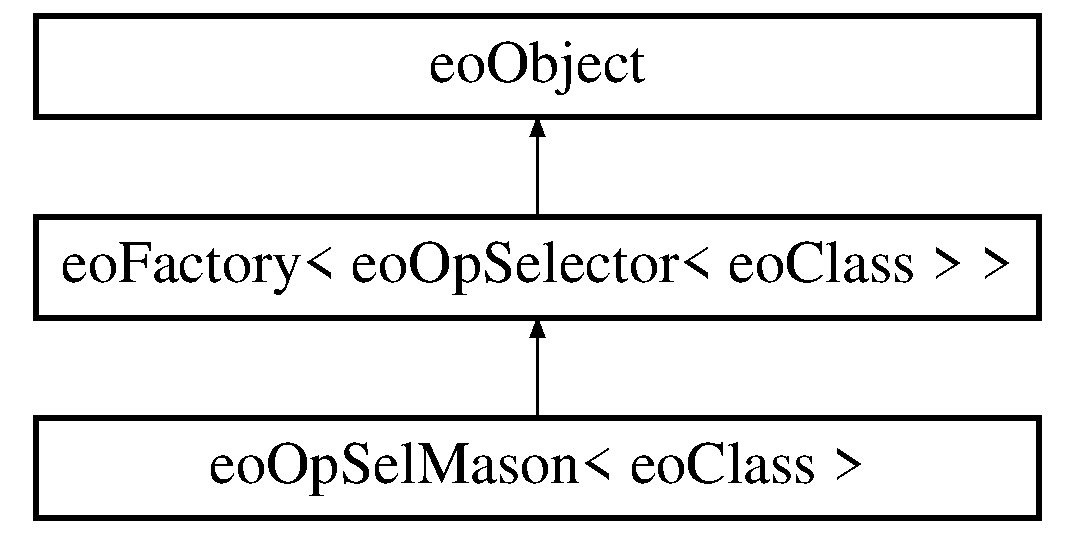
\includegraphics[height=3cm]{classeo_op_sel_mason}
\end{center}
\end{figure}
\subsection*{Public Types}
\begin{CompactItemize}
\item 
typedef std::vector$<$ {\bf eo\-Op}$<$ eo\-Class $>$ $\ast$ $>$ {\bf v\-Op\-P}\label{classeo_op_sel_mason_w0}

\item 
typedef map$<$ eo\-Op\-Selector$<$ eo\-Class $>$ $\ast$, v\-Op\-P $>$ {\bf MEV}\label{classeo_op_sel_mason_w1}

\end{CompactItemize}
\subsection*{Public Member Functions}
\begin{CompactItemize}
\item 
virtual eo\-Op\-Selector$<$ eo\-Class $>$ $\ast$ {\bf make} (std::istream \&\_\-is)
\begin{CompactList}\small\item\em Factory methods: creates an object from an std::istream, reading from it whatever is needed to create the object. \item\end{CompactList}\end{CompactItemize}
\begin{Indent}{\bf ctors and dtors}\par
\begin{CompactItemize}
\item 
{\bf eo\-Op\-Sel\-Mason} (eo\-Op\-Factory$<$ eo\-Class $>$ \&\_\-op\-Fact)\label{classeo_op_sel_mason_z15_0}

\begin{CompactList}\small\item\em constructor \item\end{CompactList}\item 
virtual {\bf $\sim$eo\-Op\-Sel\-Mason} ()\label{classeo_op_sel_mason_z15_1}

\begin{CompactList}\small\item\em destructor \item\end{CompactList}\end{CompactItemize}
\end{Indent}
\begin{Indent}{\bf eo\-Object methods}\par
\begin{CompactItemize}
\item 
virtual std::string {\bf class\-Name} () const \label{classeo_op_sel_mason_z17_0}

\begin{CompactList}\small\item\em Return the class id. \item\end{CompactList}\end{CompactItemize}
\end{Indent}
\subsection*{Private Attributes}
\begin{CompactItemize}
\item 
map$<$ eo\-Op\-Selector$<$ eo\-Class $>$ $\ast$, std::vector$<$ {\bf eo\-Op}$<$ eo\-Class $>$ $\ast$ $>$ $>$ {\bf alloc\-Map}\label{classeo_op_sel_mason_r0}

\item 
eo\-Op\-Factory$<$ eo\-Class $>$ \& {\bf operator\-Factory}\label{classeo_op_sel_mason_r1}

\end{CompactItemize}


\subsection{Detailed Description}
\subsubsection*{template$<$class eo\-Class$>$ class eo\-Op\-Sel\-Mason$<$ eo\-Class $>$}

{\bf EO}{\rm (p.\,\pageref{class_e_o})} Mason, or builder, for operator selectors. 

A builder must allocate memory to the objects it builds, and then deallocate it when it gets out of scope 



Definition at line 39 of file eo\-Op\-Sel\-Mason.h.

\subsection{Member Function Documentation}
\index{eoOpSelMason@{eo\-Op\-Sel\-Mason}!make@{make}}
\index{make@{make}!eoOpSelMason@{eo\-Op\-Sel\-Mason}}
\subsubsection{\setlength{\rightskip}{0pt plus 5cm}template$<$class eo\-Class$>$ virtual eo\-Op\-Selector$<$eo\-Class$>$$\ast$ {\bf eo\-Op\-Sel\-Mason}$<$ eo\-Class $>$::make (std::istream \& {\em \_\-is})\hspace{0.3cm}{\tt  [inline, virtual]}}\label{classeo_op_sel_mason_a0}


Factory methods: creates an object from an std::istream, reading from it whatever is needed to create the object. 

The format is op\-Sel\-Class\-Name$\backslash$ rate 1 operator1$\backslash$ rate 2 operator2$\backslash$ ...$\backslash$ Stores all operators built in a database (\#alloc\-Map\#), so that somebody can destroy them later. The Mason is in charge or destroying the operators, since the built object can180t do it itself. The objects built must be destroyed from outside, using the \#destroy\# method

Implements {\bf eo\-Factory$<$ eo\-Op\-Selector$<$ eo\-Class $>$ $>$} {\rm (p.\,\pageref{classeo_factory_a0})}.

Definition at line 65 of file eo\-Op\-Sel\-Mason.h.

The documentation for this class was generated from the following file:\begin{CompactItemize}
\item 
eo\-Op\-Sel\-Mason.h\end{CompactItemize}
